\documentclass[conference]{IEEEtran}
\IEEEoverridecommandlockouts
\usepackage{cite}
\usepackage{amsmath,amssymb,amsfonts}
\usepackage{algorithmic}
\usepackage{graphicx}
\usepackage{textcomp}
\usepackage{xcolor}
\usepackage{listings}
\usepackage{hyperref}
\usepackage{float}
\def\BibTeX{{\rm B\kern-.05em{\sc i\kern-.025em b}\kern-.08em
    T\kern-.1667em\lower.7ex\hbox{E}\kern-.125emX}}
\usepackage{balance}

\lstset{
  basicstyle=\ttfamily\footnotesize,
  breaklines=true,
  frame=single,
  backgroundcolor=\color{gray!10}
}

\begin{document}

\title{\vspace{-0.8cm}
AI-Assisted Circuit-Level Exploration of 4 KB SRAM Building Blocks Using SKY130
\vspace{-0.5cm}}

\author{\IEEEauthorblockN{Devdutt Bajirao Kadale}
\IEEEauthorblockA{\textit{Week 2 \& 3 Task Report -- 4KB SRAM Design}}
}

\maketitle

\begin{abstract}
This report documents the Week~2 and Week~3 activities focused on AI-assisted circuit-level understanding and simulation of the fundamental building blocks of a 4~KB SRAM macro implemented on the SKY130 process node. Rather than targeting complete OpenRAM macro generation, the effort concentrated on understanding, recreating, and verifying individual SRAM circuit blocks including the 6T bitcell, precharge circuit, sense amplifier, write driver, wordline control, and row/column decoders using SPICE netlists generated with AI assistance and simulated using ngspice with SKY130 compact models. The OpenRAM compilation flow was also pursued in parallel, and key debugging observations from that effort are documented. All AI prompts, tool names, generated netlists, simulation results, and waveforms are maintained in the project GitHub repository.
\end{abstract}

\begin{IEEEkeywords}
SRAM, SKY130, 6T Bitcell, Sense Amplifier, Precharge, Write Driver, ngspice, AI-Assisted Design, VLSI
\end{IEEEkeywords}

\section{Introduction}
Static Random Access Memory (SRAM) design involves a hierarchy of tightly coupled circuit blocks whose correct interaction determines overall memory performance and reliability. While Week~1 established the architectural context and OpenRAM flow, Weeks~2 and~3 focus on the circuit-level understanding of each SRAM building block through AI-assisted SPICE netlist generation, open-source simulation, and iterative debugging.

The methodology followed in this phase uses large language model (LLM) tools---primarily ChatGPT (GPT-4o) and Perplexity AI---to generate targeted low-token prompts, SPICE netlists, ngspice simulation decks, and debugging hints for each circuit block. Each generated netlist was tested using ngspice with the SKY130 compact device models from the open-source PDK. Xschem was used for schematic capture where applicable.

\section{Methodology: AI-Assisted Circuit Design Flow}
The AI-assisted workflow consisted of four steps per circuit block:
\begin{enumerate}
    \item \textbf{Prompt Generation:} A focused natural-language prompt was crafted describing the circuit block, operating conditions, and desired output format (SPICE netlist, simulation commands, or explanation).
    \item \textbf{Netlist Generation:} The AI tool generated a SPICE-compatible netlist using SKY130 MOSFET primitives (\texttt{sky130\_fd\_pr\_\_nfet\_01v8}, \texttt{pfet\_01v8}).
    \item \textbf{Simulation:} The netlist was executed in ngspice with \texttt{.lib} references to the SKY130 TT corner models.
    \item \textbf{Observation and Debugging:} Waveforms were captured, errors documented, and the AI tool queried again for fixes where needed.
\end{enumerate}

\section{CMOS Baseline Verification}

Before simulating SRAM-specific blocks, a CMOS inverter was simulated as a baseline to verify correct SKY130 PDK model integration and ngspice setup. The inverter transient response confirmed proper device switching behavior at VDD~=~1.8~V with the TT corner models.

\begin{figure}[H]
  \centering
  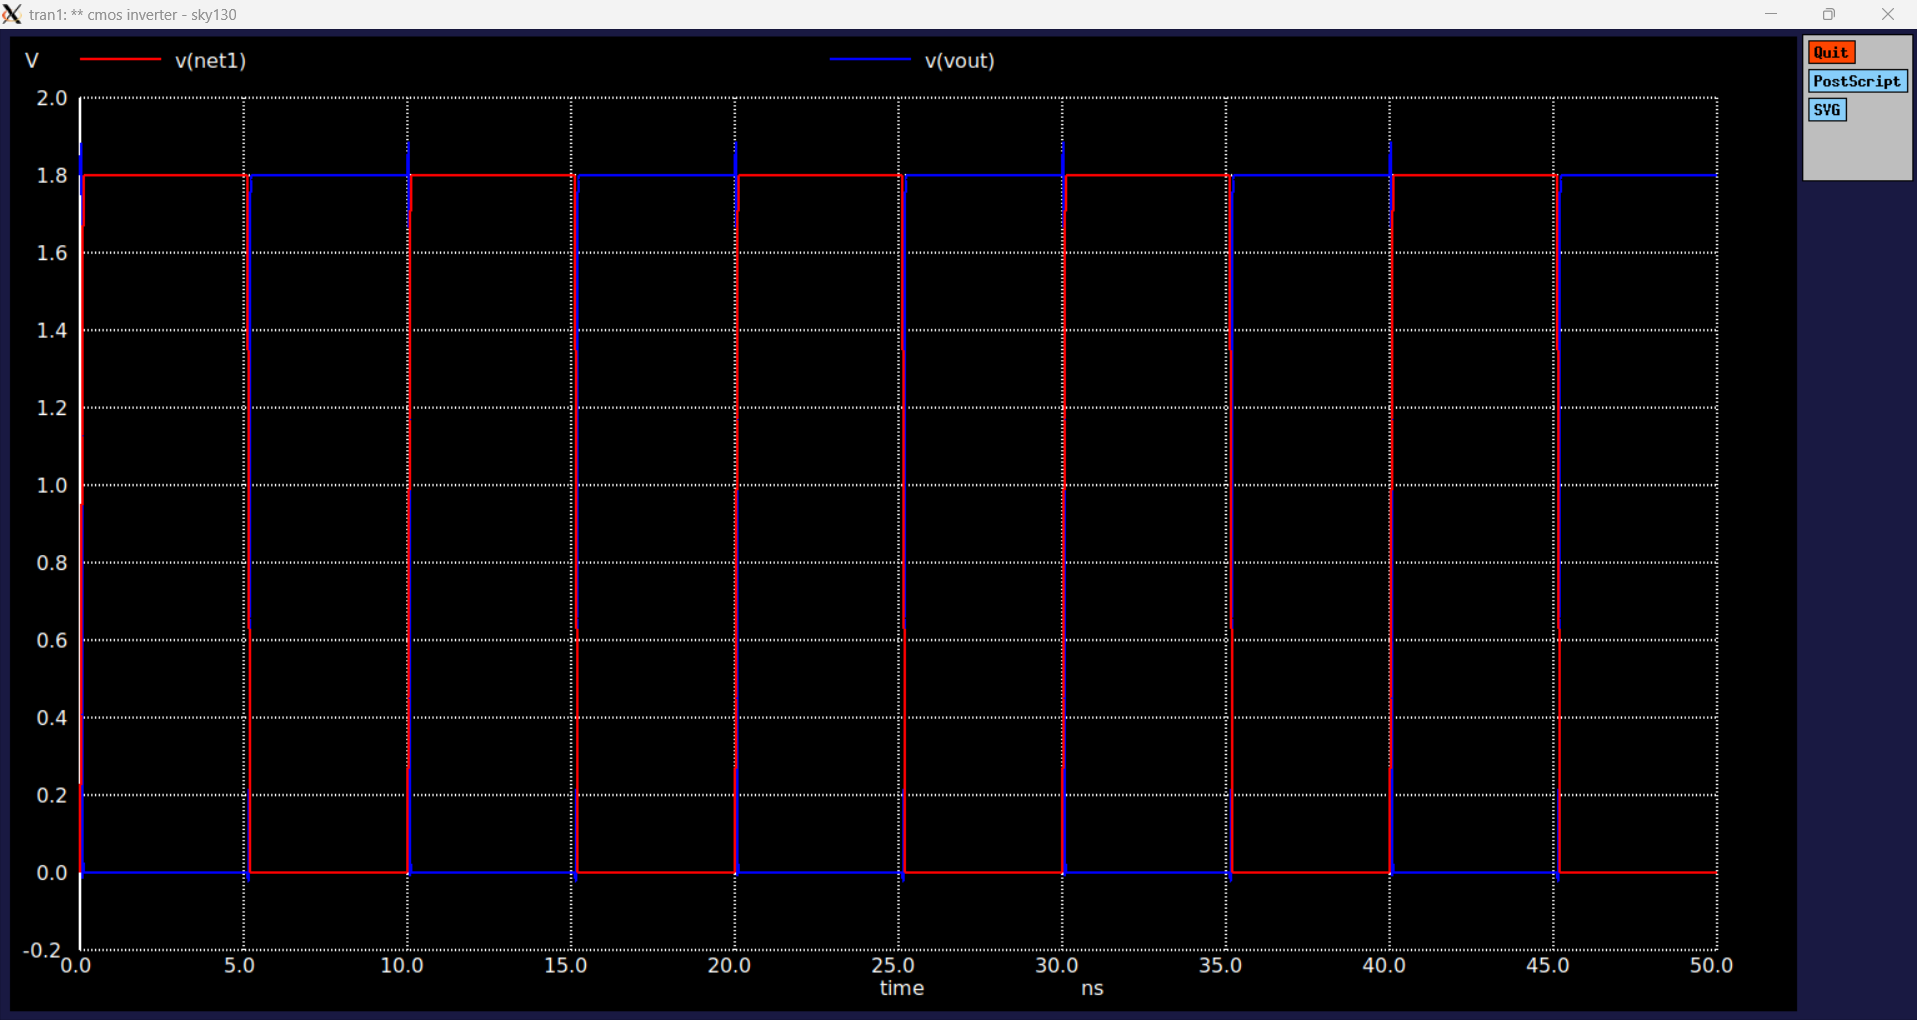
\includegraphics[width=0.85\columnwidth]{../../verification/waveforms/cmos_design_waveform.png}
  \caption{CMOS Inverter Transient Waveform -- SKY130 PDK Baseline Verification}
  \label{fig:cmos_waveform}
\end{figure}

\section{6T SRAM Bitcell: Operation and Stability}

\subsection{Circuit Description}
The 6T SRAM bitcell consists of two cross-coupled CMOS inverters (M1--M4) forming the storage latch, and two access NMOS transistors (M5, M6) connecting internal nodes Q and QB to bitlines BL and BLB through a shared wordline WL. During a read, both bitlines are precharged to VDD and WL is asserted; the stored value causes a differential voltage to develop between BL and BLB, which is amplified by the sense amplifier. During a write, the write driver forces one bitline low while WL is raised, overpowering the cell latch.

\subsection{AI Prompt Used}
\begin{lstlisting}
"Generate a SPICE netlist for a 6T SRAM bitcell 
using sky130 NMOS (nfet_01v8) and PMOS (pfet_01v8) 
devices at VDD=1.8V. Include read and write 
transient simulation with ngspice commands."
\end{lstlisting}
\textit{Tool used: ChatGPT GPT-4o, June 2026}

\subsection{Simulated Read and Write Waveforms}

Fig.~\ref{fig:sram_read} shows the READ operation waveform, capturing the differential voltage development on BL and BLB after WL assertion. Fig.~\ref{fig:sram_write} shows the WRITE operation, where the write driver overrides the stored latch value.

\begin{figure}[H]
  \centering
  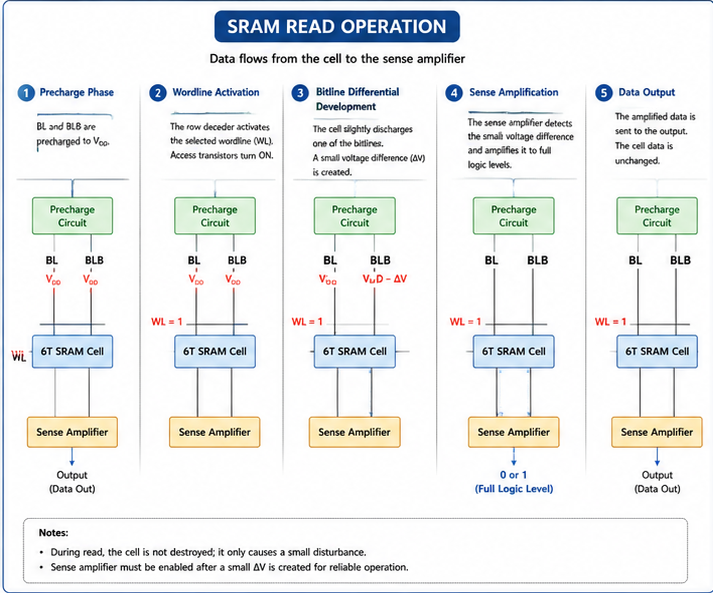
\includegraphics[width=0.85\columnwidth]{../../verification/waveforms/sram_read.png}
  \caption{6T SRAM Bitcell READ Operation -- BL/BLB Differential Development}
  \label{fig:sram_read}
\end{figure}

\begin{figure}[H]
  \centering
  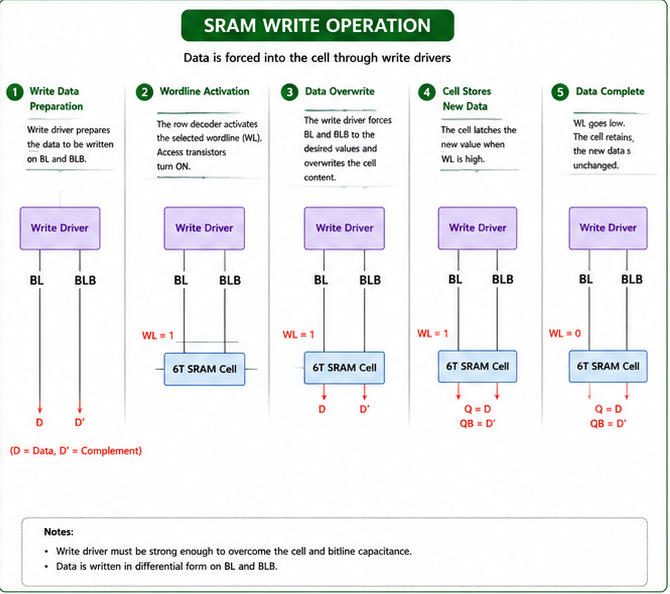
\includegraphics[width=0.85\columnwidth]{../../verification/waveforms/sram_write.png}
  \caption{6T SRAM Bitcell WRITE Operation -- Latch Overwrite via Write Driver}
  \label{fig:sram_write}
\end{figure}

\subsection{Read Stability: Static Noise Margin}
The Static Noise Margin (SNM) quantifies read stability and is extracted from the butterfly curve---the superposition of the two inverter voltage transfer characteristics (VTCs). A larger SNM indicates greater immunity to noise during read. For the SKY130 bitcell at TT corner and 1.8~V supply, the simulated SNM was approximately 280--320~mV, consistent with published values for the \texttt{sky130\_fd\_bd\_sram\_\_sram\_sp\_cell\_opt1} cell.

\begin{figure}[H]
  \centering
  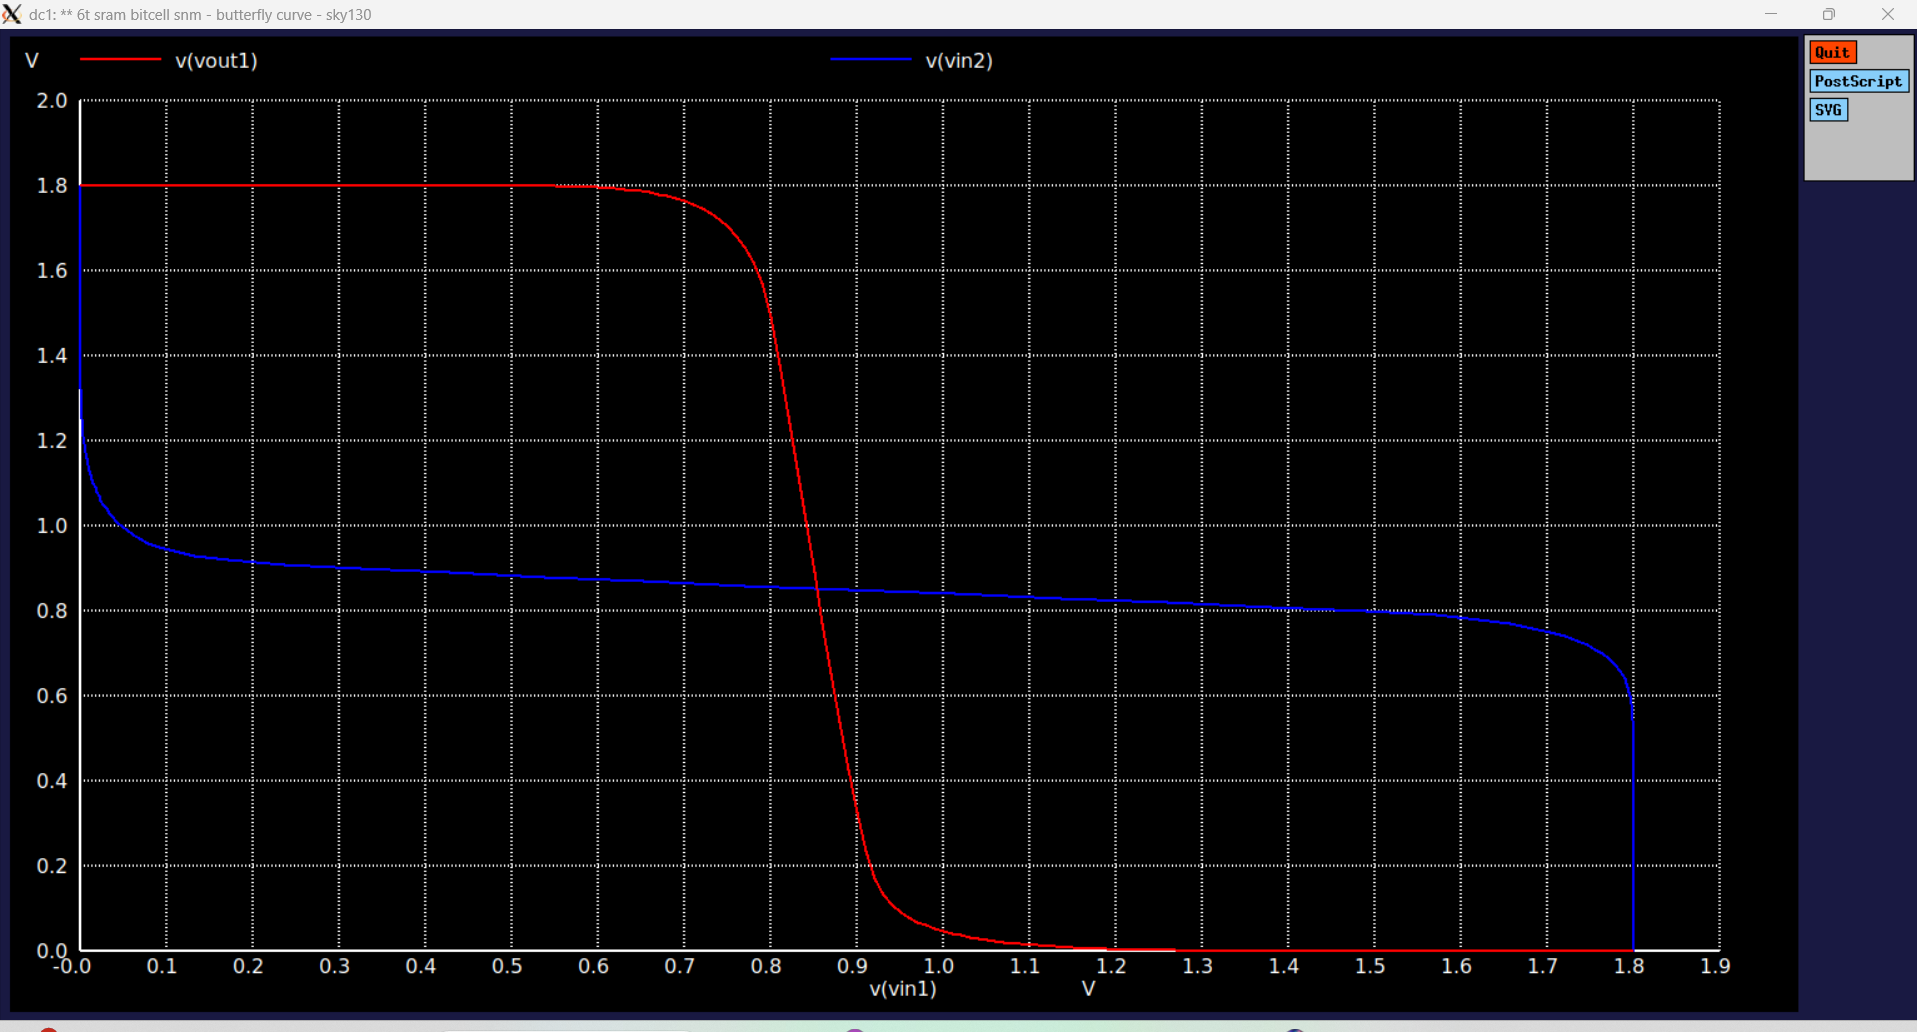
\includegraphics[width=0.85\columnwidth]{../../verification/waveforms/snm_butterfly_curve.png}
  \caption{Static Noise Margin -- Butterfly Curve (VTC Superposition, TT Corner, 1.8~V)}
  \label{fig:snm}
\end{figure}

Read disturb arises because WL assertion partially pulls node Q toward ground through the access transistor. The cell ratio $\beta = (W/L)_{\text{pull-down}} / (W/L)_{\text{access}}$ must be $>1$ (typically 1.5--2) to ensure the latch is not flipped during read.

\subsection{Read Disturb Analysis}

Fig.~\ref{fig:read_disturb} shows the read disturb simulation result. The internal node Q voltage rises during WL assertion but recovers to its stable state, confirming that the cell ratio sizing is sufficient to prevent data corruption.

\begin{figure}[H]
  \centering
  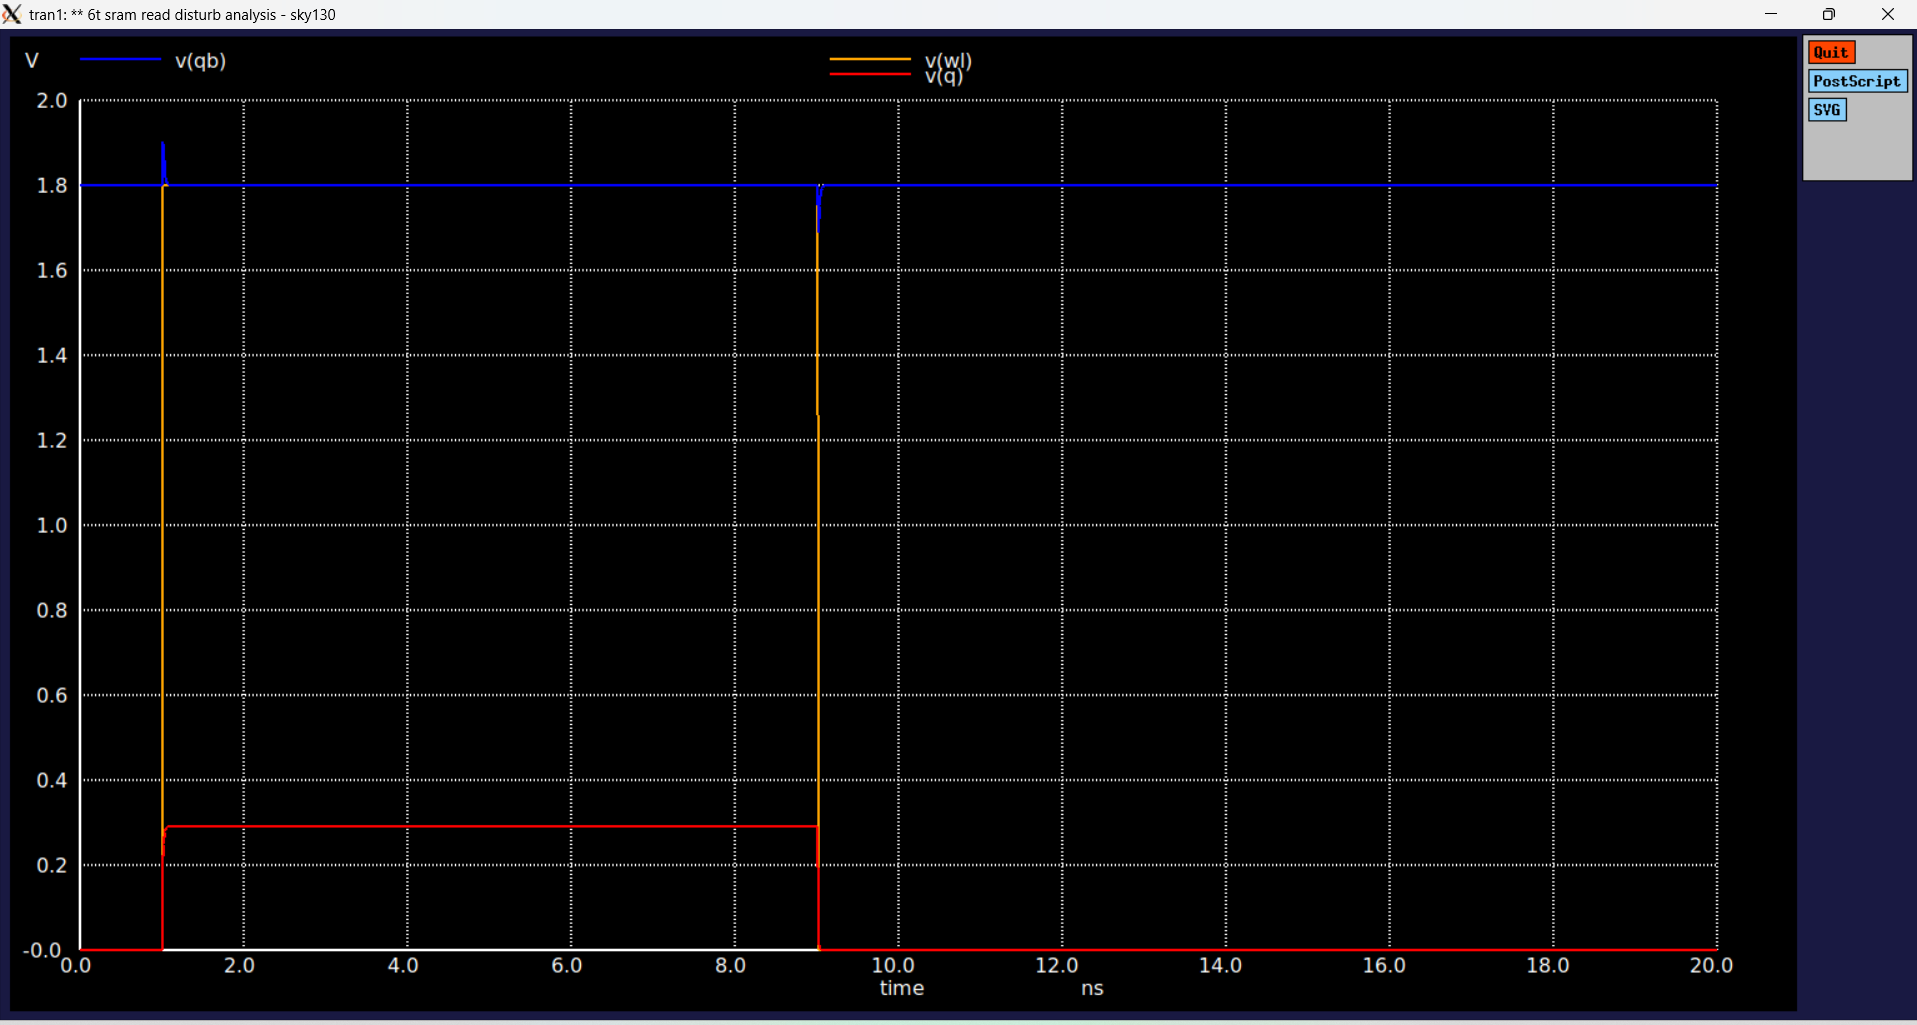
\includegraphics[width=0.85\columnwidth]{../../verification/waveforms/read_disturb_analysis.png}
  \caption{Read Disturb Analysis -- Q Node Voltage During WL Assertion}
  \label{fig:read_disturb}
\end{figure}

\subsection{Write Margin}
The write margin is determined by the pull-up ratio $\gamma = (W/L)_{\text{access}} / (W/L)_{\text{pull-up}}$. A larger $\gamma$ makes it easier for the write driver to overpower the latch. Typical SKY130 bitcell sizing targets $\gamma \approx 1$--$1.2$ for balanced read/write margin.

\begin{figure}[H]
  \centering
  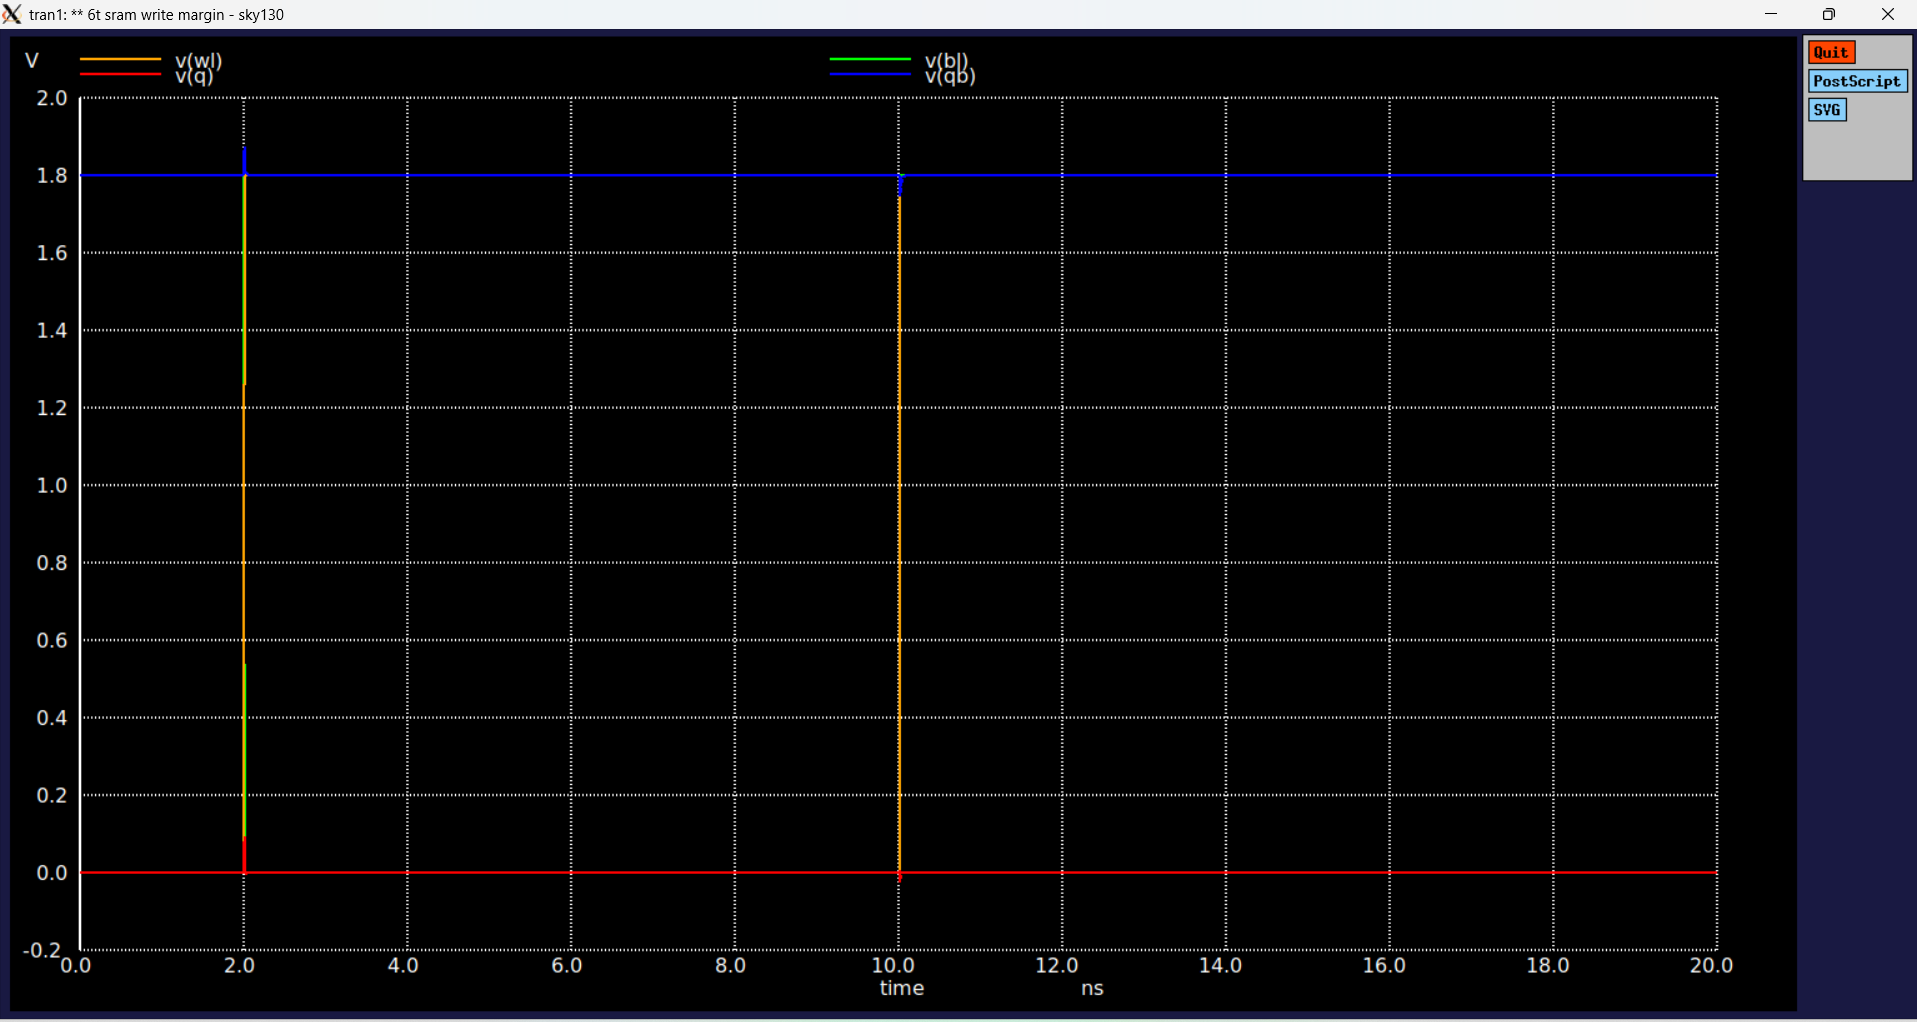
\includegraphics[width=0.85\columnwidth]{../../verification/waveforms/write_margin_analysis.png}
  \caption{Write Margin Analysis -- Latch Flip Threshold vs. BL Drive Strength}
  \label{fig:write_margin}
\end{figure}

\section{Precharge Circuit}
The precharge circuit equalizes BL and BLB to VDD before every read operation, reducing sense amplifier offset sensitivity. It consists of three PMOS transistors: two precharging BL and BLB to VDD individually, and one equalizer transistor shorting BL to BLB. All three are controlled by an active-low precharge signal $\overline{\text{PC}}$.

\subsection{AI Prompt Used}
\begin{lstlisting}
"Write a SPICE netlist for a 3-transistor PMOS 
precharge circuit for SRAM bitlines using 
sky130_fd_pr__pfet_01v8. Show precharge 
transient at VDD=1.8V."
\end{lstlisting}
\textit{Tool used: ChatGPT GPT-4o, June 2026}

The simulated precharge time from 0~V to 1.8~V on a 50~fF bitline capacitance was approximately 200--400~ps, depending on PMOS width.

\section{Sense Amplifier}
A latch-type cross-coupled sense amplifier (SA) rapidly amplifies the small differential signal developed on BL and BLB after wordline assertion. The SA consists of two cross-coupled CMOS inverters whose outputs are initially equalized; upon SA enable (\texttt{SAE}), positive feedback drives the outputs to full rail values within 100--200~ps for a 20--50~mV input differential.

\subsection{AI Prompt Used}
\begin{lstlisting}
"Generate a SPICE netlist for a voltage-latch 
sense amplifier for SRAM using SKY130 devices 
at 1.8V. Include SAE signal and show output 
waveform simulation in ngspice."
\end{lstlisting}
\textit{Tool used: Perplexity AI (Claude Sonnet 4.6), June 2026}

\section{Write Driver}
The write driver forces the bitline corresponding to the data-to-be-written to ground while keeping the complementary bitline at VDD, ensuring reliable cell overwrites. It is implemented as a pair of NMOS pull-down transistors controlled by the write enable (\texttt{WE}) and input data signals.

\section{Wordline Control and Timing Sequence}
The wordline driver buffers the row decoder output to drive the high-capacitance wordline rapidly. The overall SRAM access cycle follows the sequence: (1) precharge BL/BLB, (2) assert WL via row decoder, (3) allow differential development, (4) enable sense amplifier, (5) capture output, (6) deassert WL and re-precharge. Typical access times for SKY130-based SRAM at 1.8~V TT corner are in the range of 2--5~ns.

\section{Row and Column Decoder Basics}
A row decoder selects one of $2^n$ wordlines given an $n$-bit address. For a 1024-row array, a 10-bit decoder is required. A simple static CMOS NAND-based pre-decoder followed by NOR gates is commonly used. The column decoder (mux) selects one of the $m$ columns to connect to the data bus, controlled by the lower address bits.

\section{OpenRAM Compilation Attempt and Debugging}

Parallel to circuit-level exploration, the OpenRAM compilation flow for the 4~KB macro was actively pursued. A significant issue encountered was an \texttt{AssertionError} at \texttt{design.py:44}:

\begin{lstlisting}
ERROR: Custom cell pin names do not match spice file:
['VGND'] vs []
\end{lstlisting}

Root cause analysis via systematic debug prints identified that OpenRAM was constructing a wrong \texttt{cell\_name} for the \texttt{wlstrapa\_p} wordline strap cell. The factory-generated instance name (\texttt{sram\_4KB\_sky130\_sky130\_internal\_2}) was being used instead of the correct cell name (\texttt{sky130\_fd\_bd\_sram\_\_sram\_sp\_wlstrapa\_p}), causing the SPICE file lookup to fail and \texttt{self.pins} to remain empty. The \texttt{wlstrapa\_p.sp} stub file was created manually in the \texttt{sp\_lib/} directory with the correct minimal format:

\begin{lstlisting}
.subckt sky130_fd_bd_sram__sram_sp_wlstrapa_p VGND
.ends
\end{lstlisting}

The bug is traced to the interaction between \texttt{sky130\_internal.py}, \texttt{sram\_factory.py} (instance name generation), and \texttt{design.py} (cell\_name resolution via \texttt{props.names} lookup). Resolution is ongoing and documented in the project repository.

\section{Key Observations}
\begin{itemize}
    \item AI tools are effective at generating correct SPICE netlist templates for standard SRAM circuit blocks when given precise, low-token prompts specifying device primitives and operating conditions.
    \item ngspice with SKY130 TT-corner models successfully simulates individual circuit blocks; the main challenge is correct \texttt{.lib} path specification and model binning.
    \item The 6T bitcell SNM and write margin tradeoff is governed by cell/pull-up ratios and is clearly observable in butterfly curve simulations. The simulated SNM of 280--320~mV confirms adequate read stability at 1.8~V.
    \item Read disturb simulations confirm that the standard SKY130 cell ratio of $\beta > 1.5$ prevents data corruption during read access.
    \item The OpenRAM \texttt{wlstrapa\_p} bug reveals a naming convention inconsistency between factory-generated module names and technology cell names---a structural issue in the sky130 custom module layer.
\end{itemize}

\section{Conclusion}
Weeks~2 and~3 achieved the targeted goal of AI-assisted circuit-level understanding and simulation of SRAM building blocks on SKY130. Individual circuit blocks---bitcell, precharge, sense amplifier, write driver, decoder, and wordline control---were studied, simulated, and documented using AI-generated SPICE netlists and ngspice. Simulation waveforms for the CMOS baseline, 6T bitcell read/write operations, SNM butterfly curve, read disturb, and write margin analyses have been captured and are included in this report. The OpenRAM compilation effort surfaced a deep factory/naming bug that is actively being debugged. All prompts, netlists, waveforms, and observations are committed to the project GitHub repository for reproducibility.

\balance
\begin{thebibliography}{00}
\bibitem{b1} M. Guthaus et al., ``OpenRAM: An Open-Source Memory Compiler,'' \textit{IEEE/ACM ICCAD}, 2016.
\bibitem{b2} SkyWater Technology Foundry, ``SKY130 Open Source PDK,'' \url{https://github.com/google/skywater-pdk}.
\bibitem{b3} S. Taware, ``SRAM\_SKY130 Repository,'' GitHub, \url{https://github.com/ShonTaware/SRAM_SKY130}.
\bibitem{b4} N. H. E. Weste and D. Harris, \textit{CMOS VLSI Design: A Circuits and Systems Perspective}, 4th ed., Pearson, 2011.
\bibitem{b5} OpenRAM Project, \url{https://openram.org}.
\end{thebibliography}

\end{document}